\section{Introduction}

% Bring in the issues that our approach can address
% Describe them as problems in current simulation/emulation systems

Software defined networking (SDN) centralizes and simplifies control of network management, and has been increasingly adopted in data centers and internet exchange points\cite{B4, Meridian, SDX}.
%Software defined networking (SDN) technology separate the network control logic of the network from the distributed hardware that implementing the forwarding behaviors.
Similar to traditional computer network systems, it is crucial to perform appropriate testing and evaluation of SDN-based applications before deploying on a real system.
Researchers in the simulation community have extended various existing network simulators to support SDN capability \cite{S3F, NS3, OPNET}.
To improve experimental fidelity, researchers have also developed network emulation testbeds
(e.g., Mininet \cite{Mininet}) that utilize Linux containers over shared hardware resources and
real network stack to run high-fidelity SDN experiments.
However, container-based emulators cannot reproduce the correct behavior of a real network
with a large network topology and high traffic load because of the limited underlying physical resources.
For example, on a commodity machine with 2.98 GHz CPU, 4 GB RAM, and 3 Gbps internal bandwidth,
Mininet can only emulate a network up to 30 hosts, each with a 100 MHz CPU, 100 MB RAM and connected by 100 Mbps links \cite{ReproNetExprCBE}.
Therefore, increasing SDN testbed scalability and speed without losing the desired fidelity is essential.

%For example, a tree-topology network with depth 4 and fanout 10 consists of 1111 switches and 10000 hosts. If we want to achieve full connectivity, we need to install at least 399,960,000($\approx$ 4 * 10000 * 9999) OpenFlow rules in total. Assuming rules only have source IP address, destination IP address, inport number and outport number, each rule will consume at least 10 Bytes memory, meaning around 3.72 GB of memory are required to emulate this network. Such intensive resource requirement are not commonly satisfied by commodity low-end machines.

% State our idea
In this paper, we present a model abstraction technique to transform an SDN-based network model to a ``one-big-switch" network model.
The idea was inspired by the work on rule placement optimization in \cite{OneBigSwitchAbstraction}.
With the highly abstracted network, SDN application developers now only need to consider
simple end-to-end policy when programming a network,
and are shielded from the details on routing policy, switch memory limits,
and distributing rules across switches.
Our work applies the idea of one-big-switch abstraction for enhancing the scalability
of network simulation and emulation, while preserving the end-to-end forwarding logic.

This technique is useful if users only care about the end-to-end behavior rather than
the details within the network, such as hop-by-hop routing, or table lookup on each single switch.
\hl{
For example, one use case of our technique would be in a hybrid network simulation setting, where the user may want to run a fair large scale diversified
interconnecting subnetworks consisted of traditional TCP/IP network , SDN network, wireless network,
industry control communication network, etc.
SDN component in this scenario may not be the focus of the users' and
maintaining only the end-to-end behavior is sufficient for running the hybrid experiment.
Faster running time of the abstracted model is also beneficial for
real-time simulation in which some part(s) of the target network is emulated for higher fidelity.
Another scenario could be distributed simulation where the target network is composed of
several sub-networks owned by different parties and models of sub-networks
are shared among multiple parties.
If an user owning a local network is not willing to expose fine details of
her network to others for privacy and security reasons,
she can instead run our method on the target network and
share the resulting ``one-big-switch" model with her collaborators.
}

We develop a three-step approach to transform an SDN network to a big OpenFlow switch based network,
while still preserving the network forwarding logic equivalence.
The high-level idea is illustrated in Figure~\ref{Fig:BigSimOverview},
and the details are discussed in Section~\ref{Sec:Design}.
We first group all packets into equivalence classes by analyzing the matching fields
(e.g., source/destination MAC address/IP address/port, VLAN id, etc.)
of the OpenFlow rules installed on the switches.
An equivalence class represents a set of packets of the same network forwarding behavior.
We then create a graph-based model for each equivalence class to model its packet forwarding behavior.
Finally, we traverse all the forwarding graph models to generate rules for the big switch,
and the number of rules is largely reduced.
This way, we reduce the SDN network to a big-switch-based network to
improve the scalability of SDN simulation or emulation.

\begin{figure}[t]
\centering
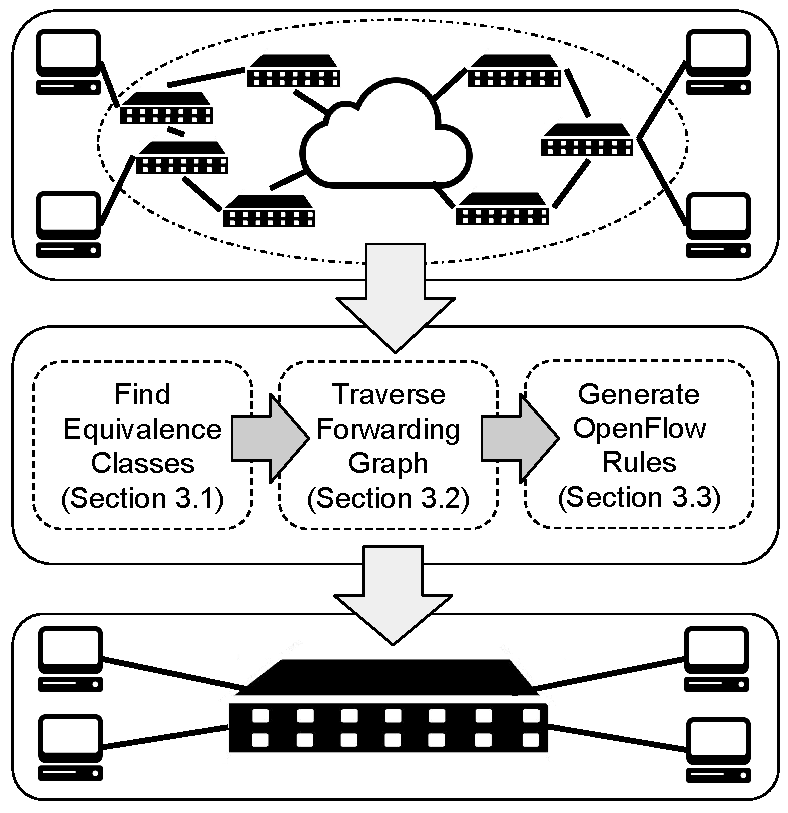
\includegraphics[scale=.6]{figures/BigSimOverview.pdf}
\caption{Transforming an SDN network to a big OpenFlow switch based network while preserving the network forwarding logic equivalence.}
\label{Fig:BigSimOverview}
\end{figure}

The reduction in the number of switches and the number of rules significantly enhances the testbed scalability and reduces the experiment running time.
For example, after abstracting a tree-topology network of depth 4 and fanout 3,
the total number of switches required to simulate is reduced from 40 to 1, and the number of rules existed in the SDN network is reduced by 89\%.
The big-switch based network model can save about
75\% to 85\% simulation execution time as compared to simulating the original network.
We can also reuse the abstracted network model.
For example, after one complete experimental run of a complex network,
users can abstract (possibly part of) the network, and reproduce the simulation results with
a much simpler configuration, including link connectivity and flow tables.
We can partition a large-scale network model, and abstract each partition in parallel.
By combining those abstracted network models, a testing platform with limited hardware resources
now can afford such network simulation/emulation experiments.
As the network state evolves, the abstracted big-switch model may also need to be frequently updated.
Our approach is lightweight. For example, we can reduce 50,000+ rules in a large tree-topology network
to 5,000+ rules in a big-switch-based network in three seconds, 
while still preserving the network forwarding rule equivalence.
In addition, our approach allows incrementally updating the big-switch model,
i.e., modifying the rules that are only affected by the current network changes.

%then why don't we just create a network with only endpoint policy and emulate it such that packet-level fidelity is preserved? In this case, we can compress the entire set of the SDN switches to single OpenFlow switch. The benefits is the much less number of switches and/or number of rules existing in the network.
%For the example mention above, we only need to start up one switch and 10000 hosts. On the single switch, we just need to install about 99,990,000 rules, only requiring less than 0.94 GB memory.
%About the "incremental update" of the Big Switch, it can be extended in our work since we use VeriFlow. But we haven't implemented it so far.%
In this work, we present a model abstraction technique to reduce networked SDN switches to a one-big-switch model. We mainly focus on preserving the end-to-end network forwarding logic.
Our long term goal is to investigate systematic model abstraction approaches that preserve end-to-end performance equivalence as well, such as latency and packet drop, to further enhance the model fidelity.

The remainder of this paper is organized as follows. Section  \ref{Sec:MotivatingExample} illustrates the problem and the approach using a simple motivating example.
Section \ref{Sec:Design} describes the details of the three-step model abstraction design.
Section 4 presents the evaluation results in terms of forwarding logic equivalence, simulation time, reduction in flow rules, and model abstraction execution time.
Section \ref{Sec:relatedwork} summarizes the related works, and Section \ref{Sec:conclusion} concludes the paper with future works.


\if 0
The precondition is that it needs to abstract the SDN network with two constraints:
\begin{itemize}
\item \textbf{Network Forwarding Rule Equivalence.}
        The forwarding behavior of any packet must be identical
        between both representations of the real network. Packets being
        forwarded through out the network (1) will also be forwarded through out
        some interface of the big switch and reach proper destination;
        (2) any modifications made by intermediate switches must be made by the
        big switch in proper order.
        Packets being dropped at some point in the network path will be drop by the
        big switch.
\item \textbf{End-to-End Latency Equivalence.}
        A packet transmitted through a series of
        switches can be seen as processed by multiple queueing systems $\mathcal{Q}$.
        Similarly, the packet processing model in a \emph{big OpenFlow switch} can
        also be modeled as a queueing system $Q$.
        The parameters of the later should be configured intelligently
        so that per packet performance metrics are as closed as possible to the ones
        in the former composite model.
        In other words, queueing delay for packet $p$, $Q(p, T)$, should be an
        function that approximates $\mathcal{Q}(p, T')$.
\end{itemize}
\fi
